\chapter{MARCO CONTEXTUAL}

El presente capítulo desarrolla las bases conceptuales y contextuales necesarias para comprender el fenómeno del lavado de dinero desde una perspectiva financiera, regulatoria y operativa, sin abordar aún los fundamentos técnicos de aprendizaje automático o profundo. Su propósito es establecer la magnitud del problema, el andamiaje normativo que lo rodea, las limitaciones de los sistemas de detección convencionales y las particularidades que las criptomonedas introducen en las tipologías de lavado. Este marco permite situar adecuadamente la motivación técnica de la tesis, esto es la detección mediante modelos basados en grafos y su explicabilidad, dentro del contexto real en el que estos sistemas deben operar.

\section{El Lavado de Dinero como Fenómeno Financiero Global}

\subsection{Definición y naturaleza del lavado de activos}

El lavado de dinero, denominado en el ámbito internacional como \textit{money laundering} (ML), es el proceso mediante el cual los fondos obtenidos a través de actividades ilícitas, entre ellas el narcotráfico, la corrupción, la trata de personas, el tráfico de armas o la evasión fiscal, son introducidos en el sistema financiero formal con la apariencia de recursos legítimos \cite{Spotlight2021Cryptocurrencies:Finances, Unagar2025SurveyXAI}. Este fenómeno constituye una amenaza de carácter transversal: no solo sustenta las economías criminales que generan los fondos de origen, sino que además erosiona la integridad de las instituciones financieras, distorsiona los mercados, reduce la confianza en los mecanismos de supervisión y debilita la gobernanza económica de los Estados \cite{Subashi2024CryptocurrenciesLaundering}.

La magnitud del lavado de activos a nivel global es difícil de cuantificar con precisión, pero las estimaciones más citadas, provenientes de la Oficina de las Naciones Unidas contra la Droga y el Delito (UNODC), sitúan el volumen de fondos lavados anualmente entre el 2\,\% y el 5\,\% del Producto Interno Bruto mundial \cite{UNODC2024EstimatingCrimes}. En términos absolutos, esto equivale a una cifra que oscila entre 800.000 millones y 2 billones de dólares estadounidenses por año. Para 2024, considerando el crecimiento del PIB global, se estima que el rango podría haber alcanzado entre 2,22 y 5,54 billones de dólares. Estas cifras subrayan que el lavado de activos no es un fenómeno residual ni marginal, sino una fuerza económica de escala sistémica que compite en magnitud con los presupuestos de defensa de naciones enteras.

Un dato particularmente alarmante es que, según estimaciones del Banco Mundial, solo alrededor del 1\,\% de los reportes de transacciones sospechosas generados a nivel global son efectivamente investigados. Esto refleja una brecha significativa entre la capacidad de generación de alertas y la capacidad institucional de procesarlas, un problema que se abordará con mayor detalle en las secciones dedicadas a los sistemas de monitoreo de transacciones.

\subsection{Las tres etapas del lavado de dinero}

La literatura financiera y criminológica coincide en que el lavado de activos se estructura típicamente en tres etapas secuenciales (Figura \ref{fig:etapas_lavado}), aunque en la práctica estas fases pueden superponerse, repetirse o adaptarse según el contexto operativo del esquema criminal \cite{FATF2012InternationalRecommendations}.

\textbf{Colocación (\textit{Placement}).} Es la primera fase del proceso, en la que los fondos ilícitos son introducidos por primera vez en el sistema financiero. Esta etapa es considerada la más vulnerable a la detección, ya que involucra el manejo directo de efectivo o activos de origen criminal. Las técnicas de colocación incluyen el fraccionamiento de depósitos en montos inferiores a los umbrales de reporte (\textit{structuring} o \textit{smurfing}), la compra de instrumentos financieros con efectivo, la utilización de negocios intensivos en efectivo como fachada y, en el contexto digital, la adquisición de criptomonedas en \textit{exchanges} con controles débiles de verificación de identidad. 

\textbf{Estratificación (\textit{Layering}).} Una vez introducidos los fondos en el sistema, la segunda etapa busca separar el dinero de su origen ilícito mediante una serie de transacciones financieras complejas diseñadas para dificultar la trazabilidad. La estratificación puede involucrar transferencias electrónicas entre múltiples cuentas bancarias en diferentes jurisdicciones, la compra y venta sucesiva de activos financieros, el uso de empresas de fachada (\textit{shell companies}), y la conversión entre diferentes tipos de instrumentos. En el contexto de las criptomonedas, esta etapa se ha sofisticado considerablemente mediante el uso de \textit{mixers}, \textit{peel chains} y puentes entre cadenas de bloques, técnicas que se analizarán en detalle en la Sección 2.5. La estratificación es considerada la fase más compleja del proceso de lavado, y es donde los mecanismos de detección enfrentan los mayores desafíos operativos.

\textbf{Integración (\textit{Integration}).} La tercera fase cierra el ciclo de lavado, reintroduciendo los fondos ya estratificados en la economía formal como recursos aparentemente legítimos. En esta etapa, los criminales pueden adquirir bienes inmuebles, invertir en negocios legítimos, comprar activos de lujo o realizar inversiones financieras convencionales. La integración es particularmente difícil de detectar, ya que los fondos han sido procesados a través de múltiples capas de transacciones y su origen criminal se encuentra sustancialmente disimulado.

\begin{figure}[htbp]
    \centering
    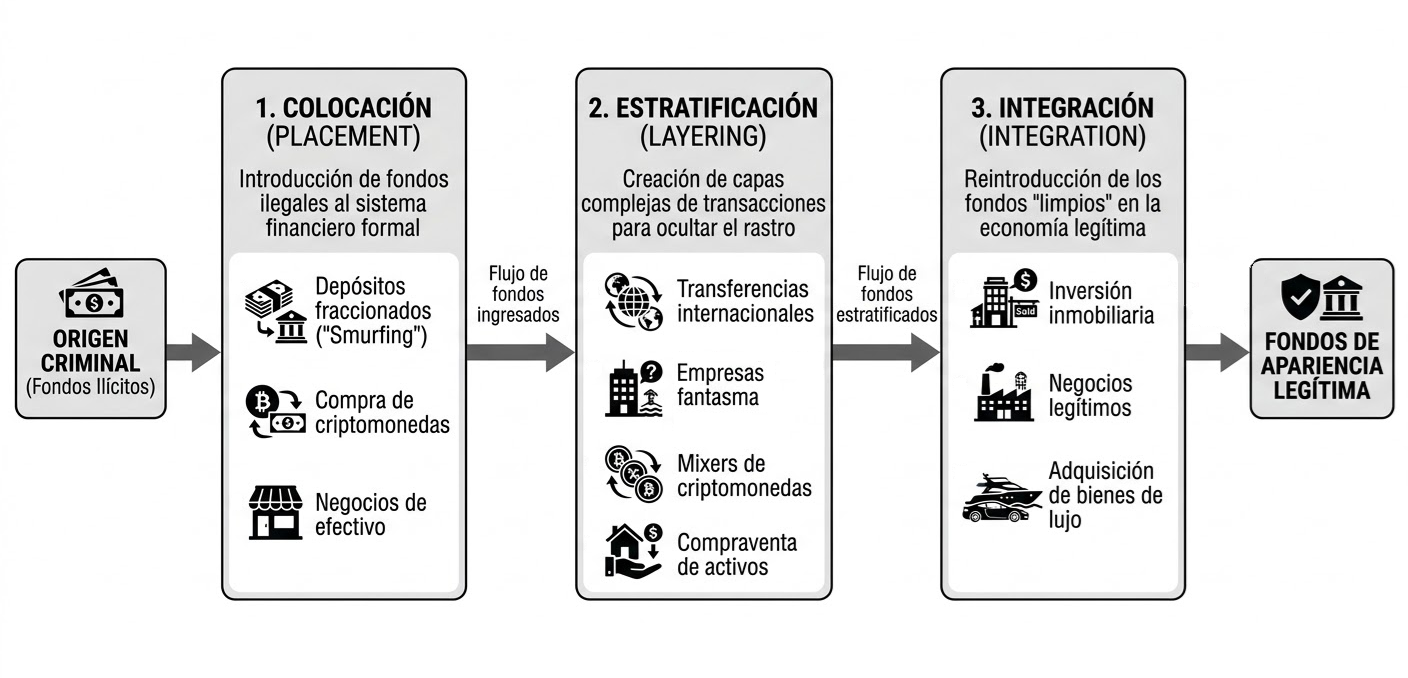
\includegraphics[width=1\textwidth]{chapter_2/images_ch2/money_laundering.png}
    \caption{Diagrama de flujo que ilustra las tres etapas clásicas del lavado de dinero (Colocación, Estratificación e Integración).}
    \label{fig:etapas_lavado}
\end{figure}

\section{Marco Regulatorio Internacional Anti-Lavado de Activos}

\subsection{El Grupo de Acción Financiera Internacional (GAFI/FATF)}

El Grupo de Acción Financiera Internacional (GAFI), conocido en inglés como \textit{Financial Action Task Force} (FATF), constituye la máxima autoridad intergubernamental a nivel mundial en la lucha contra el lavado de activos y el financiamiento del terrorismo. Fundado en 1989 por el G-7, el GAFI está conformado actualmente por 39 países miembros y ha establecido los estándares globales que rigen las políticas de prevención y detección de lavado de activos en todo el mundo \cite{FATF2012InternationalRecommendations}.

El instrumento normativo central del GAFI son las 40 Recomendaciones, un conjunto de medidas financieras, legales y de conducta que los países deben implementar para establecer sistemas efectivos de detección, prevención y represión del lavado de activos y el financiamiento del terrorismo (LA/FT). Estas recomendaciones incluyen disposiciones sobre: evaluación de riesgos, cooperación nacional, tipificación del delito, medidas de decomiso, debida diligencia del cliente (\textit{Customer Due Diligence}, CDD), registro y reporte de operaciones sospechosas, y cooperación internacional.

\subsection{Regulación de activos virtuales y la Regla de Viaje}

Con el crecimiento exponencial de las criptomonedas y los activos virtuales, el GAFI ha actualizado sus directrices para incluir a los Proveedores de Servicios de Activos Virtuales (\textit{Virtual Asset Service Providers}, VASPs) bajo el mismo marco regulatorio que las instituciones financieras tradicionales. 

Un componente clave de esta regulación es la denominada ``Regla de Viaje'' (\textit{Travel Rule}), que exige a los VASPs recopilar y transmitir datos personales tanto del emisor como del receptor para transferencias que superen los 1.000 dólares o euros. Esta disposición busca replicar en el ecosistema cripto los controles de transparencia que ya existen en las transferencias bancarias internacionales, aunque su implementación efectiva sigue siendo un desafío debido a la naturaleza descentralizada de muchas plataformas.

\subsection{Enfoque de Gestión de Riesgos del Comité de Basilea}

A nivel de supervisión bancaria prudencial, el Comité de Basilea para la Supervisión Bancaria (\textit{Basel Committee on Banking Supervision}) emitió directrices sobre la gestión sólida de riesgos relacionados con el lavado de dinero y el financiamiento del terrorismo \cite{BaselCommitteeonBankingSupervision2020SoundTerrorism}. Estas directrices establecen que los bancos deben implementar políticas y procesos robustos para mantener altos estándares éticos y prevenir el uso indebido de sus servicios para actividades criminales.

\subsection{Debida Diligencia del Cliente (KYC)}

En el centro de los marcos regulatorios AML se encuentran los procedimientos de \textit{Know Your Customer} (KYC), que constituyen el componente operativo fundamental para la verificación de identidad de los clientes y la evaluación de sus perfiles de riesgo. Los requisitos de KYC incluyen: la Debida Diligencia del Cliente (CDD) y la Debida Diligencia Reforzada (\textit{Enhanced Due Diligence}, EDD) para clientes de alto riesgo, como personas políticamente expuestas (PEPs) o clientes de jurisdicciones de alto riesgo.

\subsection{El Enfoque Basado en Riesgo}

Los estándares internacionales en materia de prevención del lavado de dinero han desplazado su recomendación desde un modelo de cumplimiento basado en reglas fijas hacia un modelo articulado alrededor del riesgo \cite{FATF2012InternationalRecommendations, BaselCommitteeonBankingSupervision2020SoundTerrorism}. Bajo este principio, conocido como enfoque basado en riesgo, cada institución financiera debe evaluar de manera continua la exposición que representan sus clientes, sus productos, sus canales de distribución y las jurisdicciones con las que opera. A partir de esa evaluación, la institución asigna sus recursos de vigilancia de forma proporcional, de modo que las relaciones de mayor riesgo reciben controles reforzados mientras que las de menor riesgo se someten a medidas simplificadas. De esta manera, el esfuerzo de cumplimiento deja de distribuirse de forma homogénea y pasa a concentrarse donde la amenaza es más plausible.

La lógica que sustenta este enfoque descansa en la eficiencia y en la efectividad del sistema de control en su conjunto. Un régimen de reglas rígidas, que exige el mismo procedimiento a todos los clientes con independencia de su perfil, tiende a saturar a los equipos de cumplimiento con revisiones de bajo valor y a generar un volumen elevado de alertas poco informativas. En contraste, al graduar la intensidad de los controles según el riesgo, la institución libera capacidad analítica para dedicarla a los casos que verdaderamente la ameritan y mejora su probabilidad de detectar operaciones sospechosas. Además, este esquema reconoce que la actividad delictiva evoluciona, por lo que ofrece la flexibilidad necesaria para reasignar recursos cuando aparecen nuevas amenazas sin necesidad de reformar por completo el marco normativo.

Sin embargo, la aplicación práctica del enfoque basado en riesgo plantea desafíos considerables que no deben subestimarse. En primer lugar, la calidad de todo el sistema depende de la solidez de la evaluación de riesgo inicial, la cual exige información confiable, criterios coherentes y personal capacitado para interpretarla, condiciones que no siempre concurren. En segundo lugar, la discrecionalidad que otorga este modelo puede convertirse en una vía para relajar controles de forma indebida, ya sea por presiones comerciales o por una lectura interesada del riesgo, lo que obliga a las autoridades a supervisar cómo se ejerce ese juicio. Por último, la naturaleza cambiante de los productos financieros, y en particular la irrupción de nuevos instrumentos digitales, dificulta clasificar el riesgo de manera estable, de modo que la evaluación requiere una actualización permanente para no quedar desfasada.

\subsection{Desafíos de la Cooperación Transfronteriza}

El lavado de dinero constituye, por su propia naturaleza, un fenómeno que desborda las fronteras de una sola jurisdicción y se despliega a través de múltiples países. Los flujos ilícitos suelen fragmentarse y desplazarse entre distintos sistemas financieros precisamente para dificultar su rastreo y para diluir el vínculo con el delito que los origina. Cuando el circuito de ocultamiento involucra criptomonedas, esta dimensión transnacional se acentúa todavía más, dado que las redes de activos virtuales operan sobre infraestructuras globales que no reconocen los límites políticos tradicionales. En consecuencia, una investigación que se limite al territorio de un solo Estado difícilmente logra reconstruir la totalidad de la cadena de transacciones.

Frente a este carácter global, la respuesta institucional permanece anclada en gran medida a la soberanía de cada país, lo que genera fricciones importantes para la cooperación. El intercambio de información entre autoridades de distintas naciones tropieza con procedimientos formales lentos, con requisitos legales heterogéneos y con celos legítimos en torno a la protección de datos y la confidencialidad. A ello se suma que los marcos legales difieren en la manera de tipificar los delitos, en las facultades que otorgan a los organismos de supervisión y en el grado de exigencia de sus controles preventivos. Estas divergencias hacen que una operación considerada sospechosa en un país pueda pasar inadvertida en otro, y que la evidencia recolectada en una jurisdicción no siempre resulte admisible o útil en la siguiente.

Los actores dedicados al lavado de dinero conocen bien estas asimetrías y las explotan de manera deliberada mediante una práctica que suele denominarse arbitraje regulatorio. En esencia, dirigen sus operaciones hacia aquellas jurisdicciones cuyos controles resultan más débiles, cuya supervisión es más laxa o cuya cooperación internacional es más limitada, con el fin de aprovechar los eslabones más frágiles de la cadena global. De este modo, un sistema de control es tan fuerte como lo permita su componente más permisivo, y los esfuerzos rigurosos de una jurisdicción pueden verse neutralizados por la existencia de refugios normativos en otra. Por esta razón, la comunidad internacional ha insistido en la armonización de estándares y en el fortalecimiento de los mecanismos de asistencia mutua, aun cuando el avance en esa dirección continúe siendo desigual y lento.

\subsection{Proveedores de Servicios de Activos Virtuales y sus Obligaciones}

Los denominados Proveedores de Servicios de Activos Virtuales (\textit{Virtual Asset Service Providers}, VASP) constituyen las entidades que ofrecen servicios de intercambio, custodia, transferencia o administración de criptoactivos por cuenta de terceros. Dentro de esta categoría se ubican, de forma destacada, los \textit{exchanges} de criptomonedas, es decir, las plataformas que permiten convertir moneda tradicional en activos virtuales y viceversa, así como intercambiar unos criptoactivos por otros. Estos proveedores ocupan una posición estratégica en el ecosistema, pues actúan como puntos de conexión entre la economía tradicional y las redes descentralizadas. Justamente por concentrar ese tránsito, se han convertido en un eslabón crítico tanto para el funcionamiento legítimo del sector como para los intentos de canalizar fondos de origen ilícito.

Consciente de esta relevancia, la regulación reciente ha incorporado a los VASP dentro del perímetro de cumplimiento en materia de prevención del lavado de dinero, sujetándolos a obligaciones análogas a las que tradicionalmente han recaído sobre los bancos. Entre esas obligaciones figuran la identificación y verificación de la identidad de sus usuarios, conocida por sus siglas en inglés como \textit{Know Your Customer} (KYC), el monitoreo continuo de las operaciones y el reporte de aquellas que resulten sospechosas ante las autoridades competentes. A ello se añade el deber de transmitir los datos que identifican al emisor y al receptor de una transferencia de activos virtuales, un requisito que replica la lógica de la información que acompaña a las transferencias bancarias convencionales \cite{FATF2012InternationalRecommendations}. Con estas exigencias, los organismos internacionales buscan cerrar la brecha que durante un tiempo permitió que el sector cripto operara al margen de los controles aplicables al resto del sistema financiero.

No obstante, trasladar estas obligaciones a un entorno descentralizado y seudónimo genera retos que carecen de equivalente directo en la banca tradicional. La debida diligencia sobre el cliente se complica cuando las direcciones que operan en una red pública no revelan por sí mismas la identidad de las personas que están detrás de ellas, de modo que un mismo actor puede controlar numerosas direcciones sin exponer un vínculo evidente. La transmisión de los datos del emisor y del receptor resulta particularmente ardua cuando una transferencia involucra billeteras autocustodiadas o proveedores situados en jurisdicciones que no imponen requisitos equivalentes, lo que fragmenta la trazabilidad de la operación. Por añadidura, la velocidad con que surgen nuevos servicios y arreglos técnicos dentro del ecosistema tiende a superar la capacidad de los proveedores para ajustar sus controles, de manera que el cumplimiento efectivo exige un esfuerzo de adaptación constante y recursos analíticos considerables.

\subsection{La Brecha entre Regulación y Capacidad Tecnológica}

Existe una tensión persistente entre el ritmo acelerado con que innova el ecosistema de las criptomonedas y la velocidad, mucho más pausada, con que las instituciones y los reguladores logran adaptar sus herramientas de detección. El sector de los activos virtuales evoluciona de forma vertiginosa, con la aparición continua de nuevos productos, protocolos y formas de intermediación que reconfiguran la manera en que circula el valor. Los marcos normativos, en cambio, requieren procesos deliberativos extensos y ciclos de reforma que difícilmente pueden seguir ese ritmo. Como resultado, cuando una norma o un control finalmente entra en vigor, las prácticas que pretendía atender ya han mutado o han sido reemplazadas por otras.

Esta asimetría se manifiesta con especial claridad en las herramientas de detección que las instituciones emplean para vigilar sus operaciones. Los sistemas tradicionales suelen apoyarse en reglas fijas y umbrales predefinidos que disparan alertas cuando una transacción cumple ciertas condiciones establecidas de antemano. Ese diseño resulta razonable frente a comportamientos conocidos, pero pierde eficacia ante tipologías nuevas que no fueron previstas al momento de formular las reglas, pues quienes buscan ocultar fondos ajustan deliberadamente sus movimientos para permanecer por debajo de los criterios de alerta. Además, un esquema de reglas rígidas tiende a producir una elevada proporción de alertas que finalmente resultan infundadas, lo que satura a los equipos de análisis y desvía su atención de los casos verdaderamente relevantes.

Ante estas limitaciones, el campo de la prevención ha comenzado a explorar enfoques de detección más sofisticados que aspiran a superar la lógica de las reglas fijas. Buena parte del interés se ha orientado hacia métodos capaces de aprovechar la estructura relacional de las transacciones, es decir, la red de vínculos que se forma cuando el dinero se desplaza de un participante a otro y que revela patrones de conexión que un examen aislado de cada operación no alcanza a captar. La intuición que motiva esta dirección sostiene que el comportamiento ilícito rara vez se agota en una transacción individual y, en cambio, deja huellas en la forma en que se organizan los flujos entre múltiples actores. En este trabajo se retoma esa intuición como punto de partida, sin adentrarse por ahora en los detalles técnicos de tales enfoques, que se desarrollan en capítulos posteriores.


\section{Sistemas Tradicionales de Monitoreo de Transacciones}

\subsection{Arquitectura de los sistemas basados en reglas}

Los Sistemas de Monitoreo de Transacciones (\textit{Transaction Monitoring Systems}, TMS) convencionales constituyen la columna vertebral tecnológica del cumplimiento AML en las instituciones financieras desde hace décadas. Estos sistemas se fundamentan en reglas deterministas, listas de vigilancia y umbrales estáticos predefinidos para identificar transacciones potencialmente sospechosas. Su lógica operativa se basa en criterios preestablecidos derivados de patrones conocidos de fraude, tales como cambios súbitos en el volumen de transacciones, ubicaciones geográficas inusuales para compras, o transacciones repetitivas dentro de períodos cortos de tiempo.

\subsection{El problema de los falsos positivos}

El problema más crítico y ampliamente documentado de los TMS convencionales es su extraordinaria tasa de falsos positivos. Según informes de la industria, entre el 90\,\% y el 98\,\% de todas las alertas generadas por los sistemas de monitoreo de transacciones corresponden a falsos positivos \cite{ForresterConsulting2023True2023}. Esto significa que la abrumadora mayoría de las alertas generadas por estos sistemas no corresponden a actividades genuinamente sospechosas, sino a transacciones legítimas.

Las consecuencias operativas de esta tasa son profundas. La carga real puede ascender hasta 22 horas por alerta cuando se consideran los procesos completos de investigación y documentación. Esta sobrecarga genera fatiga organizacional en los equipos de cumplimiento, quienes deben dedicar la mayor parte de su tiempo a perseguir señales falsas en lugar de concentrarse en amenazas genuinas.

\subsection{Costos del cumplimiento AML}

La ineficiencia de los sistemas de monitoreo se traduce directamente en costos económicos desproporcionados. El informe anual \textit{True Cost of Financial Crime Compliance} de 2023 revela que las instituciones financieras a nivel global soportan un costo total de 206.100 millones de dólares por el cumplimiento de delitos financieros \cite{ForresterConsulting2023True2023}. 

Estas cifras ilustran una paradoja fundamental: a pesar de la inversión masiva en sistemas de cumplimiento, el volumen de lavado de activos a nivel global no muestra señales claras de disminución. Como observa Kelkar (2024), los flujos financieros ilícitos continúan representando una amenaza significativa para la estabilidad económica internacional \cite{Kelkar2024AddressingStability}.

\subsection{Consecuencias Operativas y Estratégicas de la Ineficiencia}

La elevada tasa de falsos positivos no es solo un problema de costos, sino que altera la propia lógica de la función de cumplimiento. Cuando la mayor parte del tiempo de los analistas se dedica a descartar alertas irrelevantes, la capacidad de investigación se erosiona y la atención se desplaza desde los casos verdaderamente relevantes hacia un flujo constante de señales espurias. Esta saturación produce un efecto paradójico, ya que un sistema que genera demasiadas alertas incorrectas no solo falla por exceso, sino también por omisión, al aumentar la probabilidad de que operaciones ilícitas genuinas pasen desapercibidas dentro del volumen general de actividad. La ineficiencia, por tanto, compromete de forma simultánea la eficiencia económica y la eficacia detectora del sistema.

A esta dimensión operativa se suma una consecuencia estratégica que rara vez se cuantifica. La fatiga que genera el volumen de falsos positivos deteriora la moral y la retención de los equipos especializados, cuya formación es costosa y cuya experiencia es difícil de reemplazar. En un entorno donde las tipologías de lavado evolucionan con rapidez, la pérdida de talento investigativo reduce la capacidad de la institución para adaptarse a nuevas modalidades de riesgo. Por estas razones, cualquier avance que permita reducir el ruido operativo y dirigir mejor la atención analítica tiene un valor que trasciende el ahorro directo de costos, y se traduce en una mayor resiliencia del sistema de cumplimiento en su conjunto. La Figura \ref{fig:tms_vs_grafos} contrasta el monitoreo basado en reglas con el enfoque relacional basado en grafos que motiva este trabajo.

\begin{figure}[htbp]
    \centering
    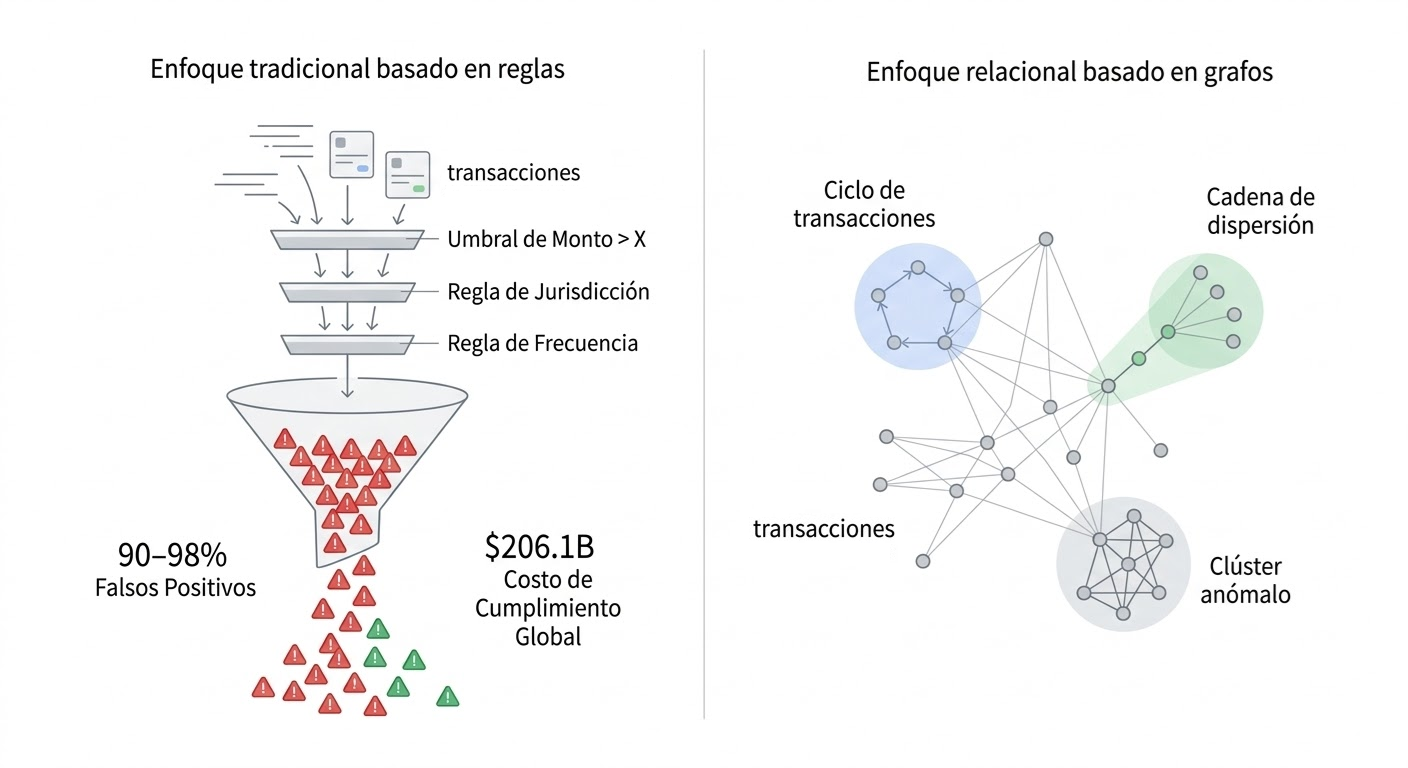
\includegraphics[width=0.9\textwidth]{chapter_2/images_ch2/enfoques_moeny_laundering.png}
    \caption{Comparación entre monitoreo transaccional basado en reglas, con umbrales estáticos y hasta 90-98\% de falsos positivos, y un enfoque relacional basado en grafos, donde las transacciones se analizan como redes para detectar patrones estructurales sospechosos (ciclos, cadenas y vecindarios anómalos).}
    \label{fig:tms_vs_grafos}
\end{figure}

\section{Criptomonedas y Delincuencia Financiera}

\subsection{Seudonimato y arquitectura descentralizada}

La emergencia de las criptomonedas ha transformado radicalmente el panorama del lavado de activos al introducir un medio de transferencia de valor que opera fuera de la infraestructura financiera tradicional \cite{Spotlight2021Cryptocurrencies:Finances}. Es importante realizar una distinción conceptual entre anonimato y seudonimato. Las criptomonedas como Bitcoin no proporcionan anonimato completo, sino seudonimato: cada transacción queda registrada de forma inmutable en la cadena de bloques y es públicamente verificable, pero las direcciones involucradas no están directamente vinculadas a identidades del mundo real \cite{Subashi2024CryptocurrenciesLaundering}.

\subsection{Magnitud de la actividad ilícita en criptomonedas}

Los datos más recientes revelan la magnitud creciente de la actividad criminal en el ecosistema cripto. Según reportes de la industria, en 2025 el volumen ilícito en criptomonedas alcanzó los 154.000 millones de dólares, un aumento sustancial respecto a años anteriores \cite{Chainalysis2025TheReport}. Como señala Europol en su informe EU-SOCTA 2025, la explotación criminal de las criptomonedas ha trascendido el ámbito del cibercrimen para permear áreas delictivas más tradicionales como el narcotráfico y el tráfico de personas \cite{Europol2025EU2025}.

\section{Tipologías de Lavado de Dinero en Criptomonedas}

\subsection{Mezcladores y servicios de ofuscación}

Los \textit{mixers} o \textit{tumblers} de criptomonedas representan una de las herramientas más utilizadas para la estratificación de fondos ilícitos. Funcionan como contratos inteligentes o servicios centralizados que reciben criptomonedas de múltiples usuarios, las combinan en un fondo común, y luego redistribuyen cantidades equivalentes a los participantes, rompiendo así el vínculo rastreable entre las direcciones de origen y destino.

\subsection{Cadenas de pelado (\textit{Peel Chains})}

Las \textit{peel chains} constituyen una técnica de lavado en la que una dirección con una cantidad significativa de criptomonedas realiza transacciones sucesivas, ``pelando'' cantidades cada vez más pequeñas hacia diferentes direcciones en cada paso. Esto distribuye los fondos gradualmente a través de una cadena de direcciones intermedias, creando una estructura transaccional larga y ramificada que complica significativamente el rastreo.

\subsection{Saltos de cadena y puentes entre \textit{blockchains}}

El \textit{chain hopping} o salto de cadena implica la conversión rápida y sucesiva de una criptomoneda a otra, generalmente utilizando diferentes \textit{blockchains}, con el propósito de dificultar el seguimiento de los fondos. Los puentes entre cadenas (\textit{cross-chain bridges}) son las herramientas tecnológicas que facilitan estas transferencias interoperables.

\subsection{Otras técnicas de lavado en criptomonedas}

Además de las técnicas principales, el \textit{smurfing} consiste en fragmentar grandes cantidades en múltiples transacciones pequeñas que quedan por debajo de los umbrales de reporte. Los \textit{exchanges} descentralizados (DEX) y las \textit{privacy coins} como Monero también incorporan protocolos que ofrecen un anonimato estructural superior. Almeida et al. (2025) documentan cómo estas estrategias de dispersión y transacciones encadenadas aprovechan la estructura de red de los ecosistemas digitales \cite{Almeida2025FromTechniques}.

La sofisticación de estas técnicas plantea un desafío directo para los sistemas de detección. Cada nueva modalidad, desde los mezcladores hasta los puentes entre cadenas, añade una capa de ofuscación que rompe la trazabilidad lineal entre el origen y el destino de los fondos. Lo que estas técnicas tienen en común es que su firma no reside en una transacción individual, sino en la configuración de relaciones que forman a través de la red, lo que refuerza la pertinencia de un enfoque estructural para su detección. Un sistema que analice cada transacción de forma aislada difícilmente distinguirá una cadena de pelado de una secuencia de pagos legítimos, mientras que un modelo que observe la topología de la red puede reconocer el patrón característico de fragmentación y dispersión que la define.

\subsection{Comparación de técnicas de lavado}

La Tabla \ref{tecnicas_lavado} sintetiza las principales técnicas de lavado de dinero empleadas en el ecosistema de criptomonedas.

\begin{table}[t]
    \centering
    \renewcommand{\arraystretch}{1.3}
    \begin{tabular}{|p{3.5cm}|p{2.5cm}|p{5.5cm}|p{2.5cm}|}
    \hline
    \textbf{Técnica} & \textbf{Etapa predominante} & \textbf{Mecanismo} & \textbf{Complejidad de detección} \\
    \hline
    \textit{Smurfing} / Estructuración & Colocación & Fraccionamiento de transacciones bajo umbrales de reporte & Media \\
    \hline
    \textit{Mixers} / \textit{Tumblers} & Estratificación & Combinación de fondos de múltiples usuarios para romper trazabilidad & Alta \\
    \hline
    \textit{Peel Chains} & Estratificación & Transferencias sucesivas de montos decrecientes a múltiples direcciones & Alta \\
    \hline
    \textit{Chain Hopping} & Estratificación & Conversión rápida entre diferentes \textit{blockchains} & Muy alta \\
    \hline
    \textit{Cross-chain Bridges} & Estratificación & Puentes tecnológicos para transferir valor entre \textit{blockchains} distintas & Muy alta \\
    \hline
    \textit{Trading} en DEX & Estratificación & Intercambio directo P2P sin intermediario centralizado & Alta \\
    \hline
    \textit{Privacy Coins} & Estrat./Integ. & Protocolos criptográficos que anonimizan transacciones por diseño & Muy alta \\
    \hline
    Compra de activos & Integración & Adquisición de bienes inmuebles, lujo con cripto convertido & Baja a Media \\
    \hline
    \end{tabular}
    \caption{Principales técnicas de lavado de dinero en criptomonedas}
    \label{tecnicas_lavado}
\end{table}

\section{Desafíos de la Detección de Fraude Financiero en el Ecosistema Cripto}

\subsection{Desafíos operativos y regulatorios}

La detección de lavado de dinero en criptomonedas enfrenta un conjunto interrelacionado de desafíos que trascienden las capacidades de los sistemas convencionales. En primer lugar, el seudonimato inherente a las criptomonedas dificulta la identificación de las partes involucradas. En segundo lugar, la naturaleza transfronteriza genera desafíos jurisdiccionales significativos. En tercer lugar, la velocidad de las transacciones en el ecosistema cripto supera ampliamente la capacidad de respuesta de los mecanismos tradicionales de monitoreo \cite{Subashi2024CryptocurrenciesLaundering}.

\subsection{La brecha entre regulación y realidad operativa}

Existe una tensión inherente entre el ritmo de innovación en el ecosistema cripto y la capacidad de los marcos regulatorios para adaptarse. Este contexto regulatorio fragmentado es particularmente relevante para la presente tesis, ya que subraya la necesidad de desarrollar herramientas de detección que puedan operar de forma efectiva basándose en los patrones estructurales y relacionales que las transacciones exhiben dentro de la red.


\section{Del Monitoreo Basado en Reglas hacia Enfoques Estructurales}

\subsection{Limitaciones fundamentales del enfoque tabular}

La limitación estructural común a los sistemas tradicionales de detección AML es su tratamiento de las transacciones como eventos aislados e independientes. Los TMS convencionales analizan cada transacción en función de sus atributos individuales sin considerar las relaciones topológicas entre las entidades involucradas.

\subsection{Transacciones financieras como grafos}

La representación de redes transaccionales como grafos ofrece un marco conceptual natural para abordar las limitaciones del enfoque tabular. En este paradigma, las entidades financieras se representan como nodos del grafo, mientras que las transacciones entre ellas constituyen las aristas. Esta formulación permite capturar propiedades fundamentales de las redes financieras que son invisibles para los modelos tabulares.

Esta representación relacional habilita un conjunto de análisis que el enfoque tabular no puede realizar. La posición de una transacción dentro de la red, medida por indicadores de centralidad, revela su importancia estructural más allá de sus atributos individuales. Los patrones de conectividad permiten identificar configuraciones características del lavado, como cadenas de intermediación, ciclos de reintegración o estructuras de dispersión en las que un origen reparte fondos hacia numerosos destinos. La propagación de información a través de la red hace posible que la clasificación de una transacción incorpore el contexto de sus vecinos, de modo que una operación individualmente benigna pueda señalarse como sospechosa por la compañía que mantiene dentro del grafo. Estas capacidades explican por qué el modelado basado en grafos se ha consolidado como el enfoque de referencia para la detección estructural de actividad ilícita en criptomonedas.

No obstante, la perspectiva de red introduce también desafíos que el enfoque tabular no enfrenta. La calidad de las conclusiones depende de la calidad de las conexiones observadas, y una red incompleta o ruidosa puede inducir a error tanto al clasificador como a las explicaciones que de él se derivan. La dispersión de la red, es decir la escasez de conexiones por nodo, limita la información contextual disponible y, como se documenta en el Capítulo 4, puede llegar a impedir que las explicaciones estructurales sean informativas. Reconocer estas limitaciones desde el marco contextual es necesario para interpretar con prudencia los resultados que las técnicas basadas en grafos producen, y anticipa la necesidad de un eje experimental complementario que permita evaluar aquello que un grafo disperso no deja medir.

\subsection{El Elliptic Dataset como referente de datos reales}

En el contexto específico de la detección AML en Bitcoin, el \textit{Elliptic Dataset} se ha consolidado como uno de los conjuntos de datos de referencia más importantes. El trabajo pionero de Weber et al. (2019) demostró que la representación de la red de transacciones Bitcoin como un grafo permite capturar patrones estructurales que los modelos tabulares no pueden identificar \cite{Weber2019Anti-MoneyForensics}. Unagar y Borisaniya (2025) confirman que los métodos basados en grafos representan el estado más avanzado de la técnica para este dominio \cite{Unagar2025SurveyXAI}.

\subsection{Hacia la necesidad de modelos explicables}

En un entorno donde las decisiones automatizadas pueden derivar en el bloqueo de cuentas o investigaciones con implicaciones jurídicas significativas, la capacidad de explicar y justificar las alertas generadas es tan importante como su precisión predictiva. Esto implica que los modelos de detección deben producir no solo una clasificación binaria, sino también una justificación comprensible del porqué. Este requisito conecta directamente con el objeto central de la presente tesis: la evaluación de la estabilidad de los métodos de explicabilidad (XAI) aplicados a modelos de grafos para detección AML.
